\subsection{Integrating the model checker and the theorem prover}
\label{sub:integrating}
Figure~\ref{Fig.3vdvinstance} presents an instance of \NAME\ obtained as an integration of a model checker for PKSs and LTL based on three-valued semantics and the theorem prover presented in Section~\ref{sec:adapting}. The circled numbers in Figure~\ref{Fig.3vdvinstance} indicate how this specific instance is plugged into \NAME\ in Figure~\ref{Fig.3vdv}.






The three-valued model checker presented in Section~\ref{sec:preliminaries} is used by \NAME\  to check the satisfaction of the property of interest.
Specifically, it runs twice a classical two-valued model checker, considering first the optimistic approximation $M_{opt}$, then the pessimistic approximation $M_{pes}$ of the PKS $M$.
When $M_{opt}$ is evaluated, if a counterexample is found, this is returned as output of \NAME .
Otherwise, \NAME\ verifies $M_{pes}$. 
If the property is satisfied, it means that no violating nor possibly violating behaviors have been identified.
Thus, \NAME\ executes the theorem prover that produces a proof that explains why no counterexample has been found in the pessimistic approximation.
Otherwise, the property is possibly satisfied.
In this case, \NAME\ returns the possible counterexample and runs the theorem prover on $M_{opt}$ to compute a proof that specifies why a definitive counterexample has not be found.




\begin{figure}[t]
\begin{center}         
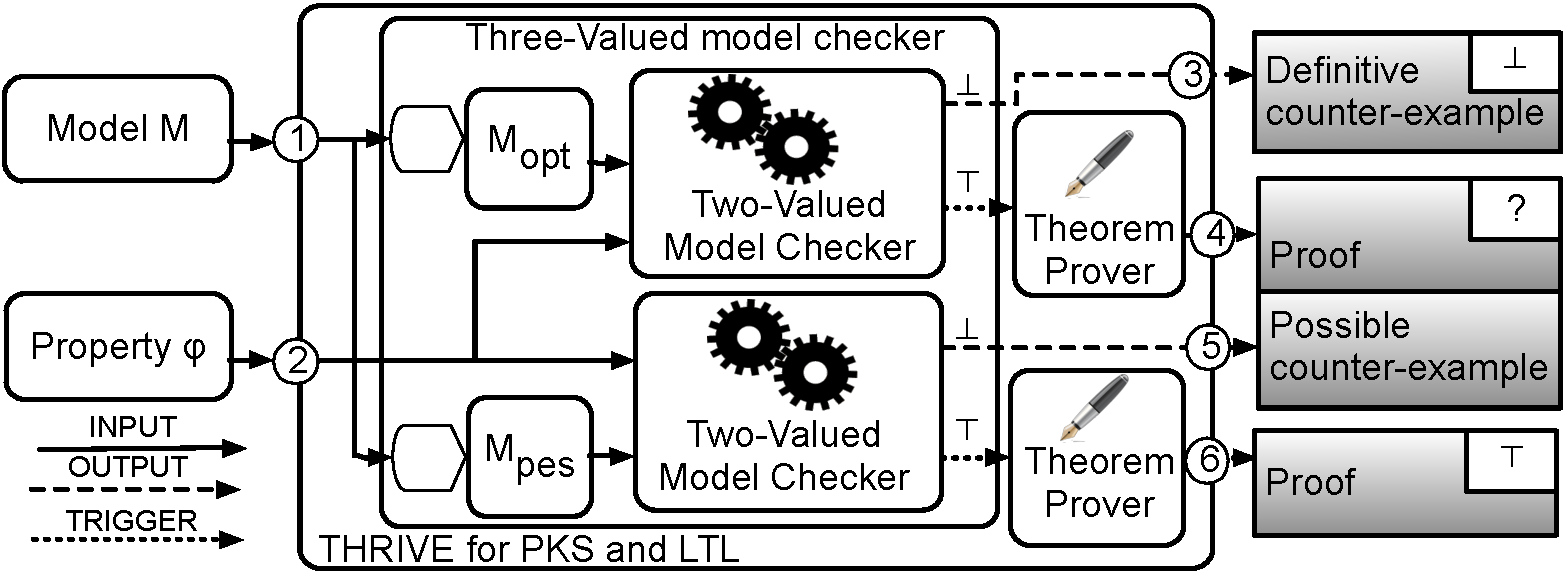
\includegraphics[width=\linewidth]{./images/atvaFigPKS.pdf}
\end{center}
\caption{\NAME\ for PKS and LTL.}  
\label{Fig.3vdvinstance}
\end{figure}



\textbf{Example}
%\emph{Consider properties $\phi_1$, $\phi_2$ and $\phi_3$ of the crossing semaphore example. They are satisfied, possibly satisfied and not satisfied, respectively, by the model $M$ of Figure~\ref{fig:model}.}
\emph{Properties $\phi_1$, $\phi_2$ and $\phi_3$ of the crossing semaphore example are satisfied, possibly satisfied and not satisfied by the model $M$ of Figure~\ref{fig:model}.}

\emph{
Property $\phi_2$.
The products between the optimistic and pessimistic approximation of the model $M$ and the BA automaton $\mathcal{A}_{\neg \phi_2}$ are presented in Figures~\ref{fig:productOpt} and~\ref{fig:productPess}.
\NAME\ explores $I_{pes}$ and returns the possible counterexample $(s_0, s_2)^\omega$.
Specifically,  by looping an infinite number of times on states $s_0$ and $s_2$ the green light is never turned on.
Since the property $\phi_2$ is possibly satisfied, the search of a definitive counterexample in the product automaton $I_{opt}$ (Figure~\ref{fig:productOpt}) fails.
%\NAME\ uses the product automaton $I_{opt}$ to compute a proof that explains the motivation.
%The obtained proof is presented in Table~\ref{table:proof}.
\NAME\ uses the product automaton $I_{opt}$ to compute a proof (Table~\ref{table:proof}) that explains the motivation.
The states that are analyzed in different steps are circled  in Figure~\ref{fig:productOpt} through different grey frames.
(\emph{Step1}). \NAME\ analyzes the failed states.
Given a failed state $\langle s, q \rangle$, since in this state the search for a counterexample fails, the formula associated with the state $q$ of $\mathcal{A}_{\lnot\phi_2}$ holds in $s$.
For example, since the state $\langle s_1, q_1 \rangle$ of $I_{opt}$ is a failed state, the formula $green \LTLor \LTLnext \LTLfinally green$ (valid in $q_1$) is satisfied by the model state $s_1$.
This formula is effectively true in $s_1$ since the green light is on.
(\emph{Step2}). Since all the successors of $\langle s_0, q_1 \rangle$ satisfy $green \LTLor \LTLnext \LTLfinally green$, it is possible to deduce that this property is also satisfied in $s_0$.
(\emph{Step3}). 
%The induction rule is applied considering the strongly connected component  $\left \{ \langle s_0, q_0 \rangle, \langle s_1, q_0 \rangle, \langle s_2, q_0 \rangle \right \}$.
%The rule allows to conclude that $s_0$ satisfies the property $\LTLnext \LTLglobally \LTLfinally green$.
The induction rule is applied considering the strongly connected component  $\left \{ \langle s_0, q_0 \rangle, \langle s_1, q_0 \rangle, \langle s_2, q_0 \rangle \right \}$ and  allows concluding that $s_0$ satisfies the property $\LTLnext \LTLglobally \LTLfinally green$.
(\emph{Step4}). \NAME\ applies the conjunction rule to $s_0$.
Since $s_0$ satisfies both $\LTLnext \LTLglobally \LTLfinally green$ and $green \LTLor \LTLnext \LTLfinally green$, it is possibly to deduce that $s_0$ satisfies the property $\phi_2$.
This provides an interesting insight to the designer: if she/he turns the green light on in $s_2$ the property becomes satisfied. The proof clearly states why.}

\emph{Property $\phi_3$. \NAME\ returns the counterexample $(s_0, s_1)^\omega$.
The counterexample specifies that by looping an infinite number of times on states $s_0$ and $s_1$ the green light is not permanently  on after the red. }

\emph{Property $\phi_1$. \NAME\  produces a proof that highlights how and why a definite counterexample is not found in the graph. First, it identifies the states $\langle s_0, q_1 \rangle$ and $\langle s_2, q_1 \rangle$ as failed. The conclusions found on these states are propagated to the state $\langle s_1, q_1 \rangle$. All the successors of the SCC formed by the product states related to the property state $q_0$ are analyzed. Finally, conclusions are drawn also on this SCC. 
The proof is omitted for space reasons.
}



\begin{table}[t]
\centering
\caption{Proof that $\phi_2$ is not violated.}
\label{table:proof}
\begin{tabular}[b]{ | P{2.5cm} | P{2.1cm} | P{3.3cm} | P{3cm} |  }
\hline
\emph{Step 1} &
\emph{Step 2} &
\emph{Step 3} &
\emph{Step 4}\\
\hline
%%\multicolumn{4}{|c|}{Steps}  \\
%% \hline
\textbf{Fail} & 
\textbf{Successors} &
\textbf{Induction} &
\textbf{Conjunction}\\
 \hline
\mbox{ $\langle s_2,q_1\rangle, \langle s_1,q_1\rangle$}
 &
 $\langle s_0,q_1\rangle$ 
 &
 $\mathcal{X}=\{\langle s_0,q_0\rangle,$ $ \langle s_1,q_0\rangle,\langle s_2,q_0\rangle\}$\newline
 $Exit(\mathcal{X})=\{\langle s_0,q_1\rangle, $ $ \langle s_1,q_1\rangle,\langle s_2,q_1\rangle\}$
 &
The initial state $s_0$ \\	
 \hline
  \inferrule{\langle s_1,q_1 \rangle  \in \mathcal{F}(I_{opt})\\
 \langle s_2,q_1 \rangle \in \mathcal{F}(I_{opt})
}
{ s_1, s_2\models g \LTLor \LTLnext \LTLfinally g }
  & 
 \inferrule{s_0\rightarrow\{s_1,s_2\} \\
 s_1\models g \LTLor \LTLnext \LTLfinally g \\
 s_2\models g \LTLor \LTLnext \LTLfinally g }
 {s_0\models g \LTLor \LTLnext \LTLfinally g} 
  &
\mbox{   \inferrule{ 
 s_0,s_1,s_2\models g \LTLor \LTLnext \LTLfinally g \\
s_0\rightarrow \{s_1,s_2 \} \\\\
 s_1\rightarrow \{s_0 \} \\\\
 s_2\rightarrow \{s_0 \}   
   }
{s_0,s_1,s_2\models \LTLnext \LTLglobally \LTLfinally g }}
  &
\inferrule{
 s_0\models \LTLnext \LTLglobally \LTLfinally g \\
  s_0\models g \LTLor \LTLnext \LTLfinally g \\
 \LTLnext \LTLglobally \LTLfinally g \LTLand  (g \LTLor  \LTLnext \LTLfinally g)\rightarrow \phi_2 }
 {s_0\models \phi_2}
\\  
\hline

\end{tabular}
\end{table}
